\chapter{Sliding Phase}
When the state of the system is finished with its reaching phase, the system enters the sliding phase. The sliding phase
are reached when the systems slides along the manifold heading towards the equilibrium point in origin. One way to do
this is with a control law as:
\begin{equation}
  u = -\beta \left( \vect{x} \right)\up{sign}(s)
\end{equation}
Where:
\begin{alignat}{5}
       & \beta (\vect{x}) & \hspace{1cm} & \quad\text{is a control gain function} \hspace{1cm} &  & \nonumber \\ 
       & s                & \hspace{1cm} & \quad\text{is the manifold} \hspace{1cm}            &  & \nonumber \\ 
\end{alignat}
And:
\begin{equation}
  \up{sign}(s) =
  \begin{cases}
    -1 & \quad s < 0 \\
     0 & \quad s = 0 \\
     1 & \quad s > 0
  \end{cases}
\nonumber
\end{equation}
This strategy can, however, give rise to a fair amount of chattering in the system. To alleviate this we define a
constant, $\epsilon$. The constant $\epsilon$ is used to define a region close to the sliding surface where, when
within, the sign$()$ function is replaced with an approximation of a discontinous function - a saturation function.
\begin{equation}
  u = -\beta\left( \vect{x} \right) \up{sat}\left( \frac{s}{\epsilon} \right)
\end{equation}
Where:
\begin{equation}
  \up{sat}\left( \frac{s}{\epsilon} \right) =
  \begin{cases}
    \frac{s}{\epsilon} &\quad \text{if $\vert\frac{s}{\epsilon}\vert$ $\leq$ 1} \\[2mm]
    \up{sign}\left( \frac{s}{\epsilon} \right) &\quad \text{if $\vert \frac{s}{\epsilon}\vert$ $>$ 1}
  \end{cases}
\end{equation}

\begin{figure}[H]
  \centering
  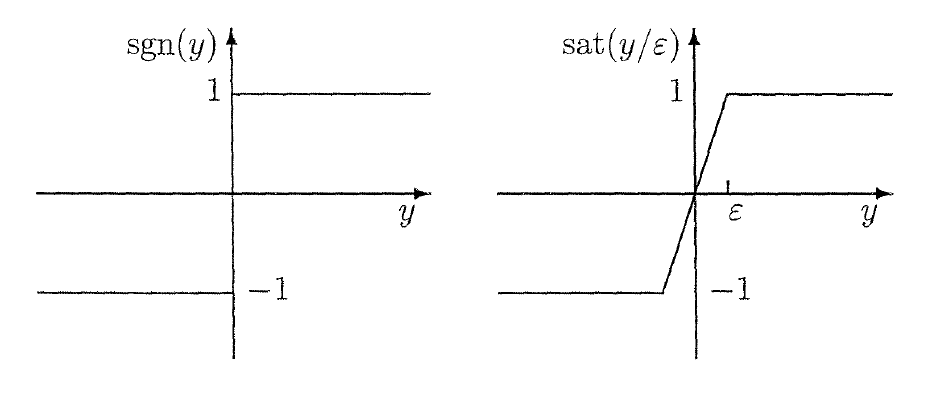
\includegraphics[width=0.6\textwidth]{saturation}
  \caption{Signum function (left) and the saturation function (right).}
  \label{fig:sign_sat}
\end{figure}


